\documentclass{article}
\usepackage[utf8]{inputenc} % Obsługuje kodowanie UTF-8
\usepackage[T1]{fontenc}    % Obsługuje czcionki w kodowaniu T1
\usepackage{graphicx}
\usepackage{amsmath}
\usepackage{float}
\usepackage{tikz}
\usepackage{pgfplots}
\usepackage{listings}
\usepackage{xcolor}
\usepackage{makecell}

\lstset{ 
	language=C++,
	backgroundcolor=\color{black!5},
	basicstyle=\footnotesize\ttfamily,
	keywordstyle=\color{blue},
	commentstyle=\color{green!50!black},
	stringstyle=\color{red!70!black},
	numbers=left,
	numberstyle=\tiny\color{gray},
	stepnumber=1,
	frame=single,
	rulecolor=\color{black!30},
	tabsize=4,
	breaklines=true,
	breakatwhitespace=false,
	showspaces=false,
	showstringspaces=false,
	showtabs=false,
	}


\title{Analiza algorytmów sortujących}
\author{Tomasz Warzecha}
\date{}

\begin{document}
	
	\maketitle
	
	\section{Wstęp}
	W sprawozdaniu moim celem jest analiza i porównanie wydajności trzech głównych algorytmów sortowania wraz z ich modyfikacjami. Insertion sort, merge sort, heap sort zostały zaimplementowane, tak aby przeprowadzić na nich różne testy wydajności. Badania te skupiają się na generowaniu losowych danych, które następnie są używane do obliczenia czasu wykonania algorytmów oraz liczby operacji takich jak przypisania i porównania. Wyniki tych testów mają na celu porównanie algorytmów, a także pokazanie różnic między teoretycznymi, a praktycznymi wynikami. 
	
	\section{Implementacja algorytmów} 
	Algorytmy zostały zaimplementowane zgodnie z klasycznymi wersjami algorytmów sortujących, korzystając z pseudokodów zamieszczonych na stronie przez prof. Szymona Żeberskiego. Wprowadzone zostały także modyfikacje, które delikatnie zmieniają działanie algorytmów. Algorytmy zostały zaimplementowane dla tablic z liczbami typu \texttt{float}.
	
	\paragraph{Najciekawsze fragmenty kodu\\}
	Poniżej przedstawię najciekawsze fragmenty kodu, wraz z objaśnieniami, tak aby łatwiej zrozumieć działanie algorytmów. 
	
	\begin{itemize}
		\item \textbf{Insertion Sort:} Algorytm sortowania przez wstawianie polega na wybieraniu kolejnych elementów z nieposortowanej części tablicy i wstawianiu ich w odpowiednie miejsce wśród już posortowanych elementów.
		\begin{lstlisting}
for(int i = 1; i < n; i++) {
	float key = A[i];
	int j = i - 1;
	while(j >= 0 && A[j] > key) {
		A[j + 1] = A[j];
		j = j - 1;
	}
	A[j + 1] = key;
}
		\end{lstlisting}
		W powyższym kodzie zmienna \texttt{key} przechowuje aktualnie wybrany element do wstawienia. Pętla \texttt{while} przesuwa większe elementy o jedno miejsce w prawo, aż znajdzie odpowiednią pozycję dla elementu \texttt{key}.
		
		\item \textbf{Merge Sort:} Sortowanie przez scalanie to metoda, która dzieli tablicę na dwie części, sortuje je osobno, a następnie scala w jedną posortowaną całość.
		\begin{lstlisting}
if (L[i] <= R[j]) {
	A[l] = L[i];
	i++;
} else {
	A[l] = R[j];
	j++;
}
		\end{lstlisting}
		Tutaj, podczas scalania dwóch posortowanych podtablic \texttt{L} i \texttt{R}, wybierany jest mniejszy element i dodawany do głównej tablicy \texttt{A}. W ten sposób elementy są umieszczane we właściwej kolejności.
		
		\item \textbf{Heap Sort:} Sortowanie przez kopcowanie wykorzystuje strukturę danych zwaną kopcem, aby organizować elementy w taki sposób, że największy lub najmniejszy element można łatwo usunąć i umieścić na końcu tablicy.
		\begin{lstlisting}
void heapify(float A[], int n, int i) {
	int largest;
	int l = left(i);
	int r = right(i);
	
	if (l < n && A[l] > A[i]) {
		largest = l;
	} else {
		largest = i;
	}
	
	if (r < n && A[r] > A[largest]) {
		largest = r;
	}
	
	if (i != largest) {
		float temp = A[i];
		A[i] = A[largest];
		A[largest] = temp;
		heapify(A, n, largest);
	}
}

		\end{lstlisting}
		Funkcja \texttt{heapify} zapewnia, że poddrzewo naszego kopca jest poprawnie ułożone - wyszukuje największy element spośród korzenia i jego dzieci, a następnie zamienia elementy, jeśli korzeń nie jest największy.
	\end{itemize}
	
	
	\section{Porównanie algorytmów}
	\subsection{Porównanie czasów działania}
	Porównanie czasów wykonania algorytmów na różnych długościach tablic: od 10 do 100010. Liczby zostały przydzielone losowo z zakresu (-1000;1000). Dane zostały przedstawione na wykresie poniżej.
	
	\begin{figure}[H]
	     \centering
	     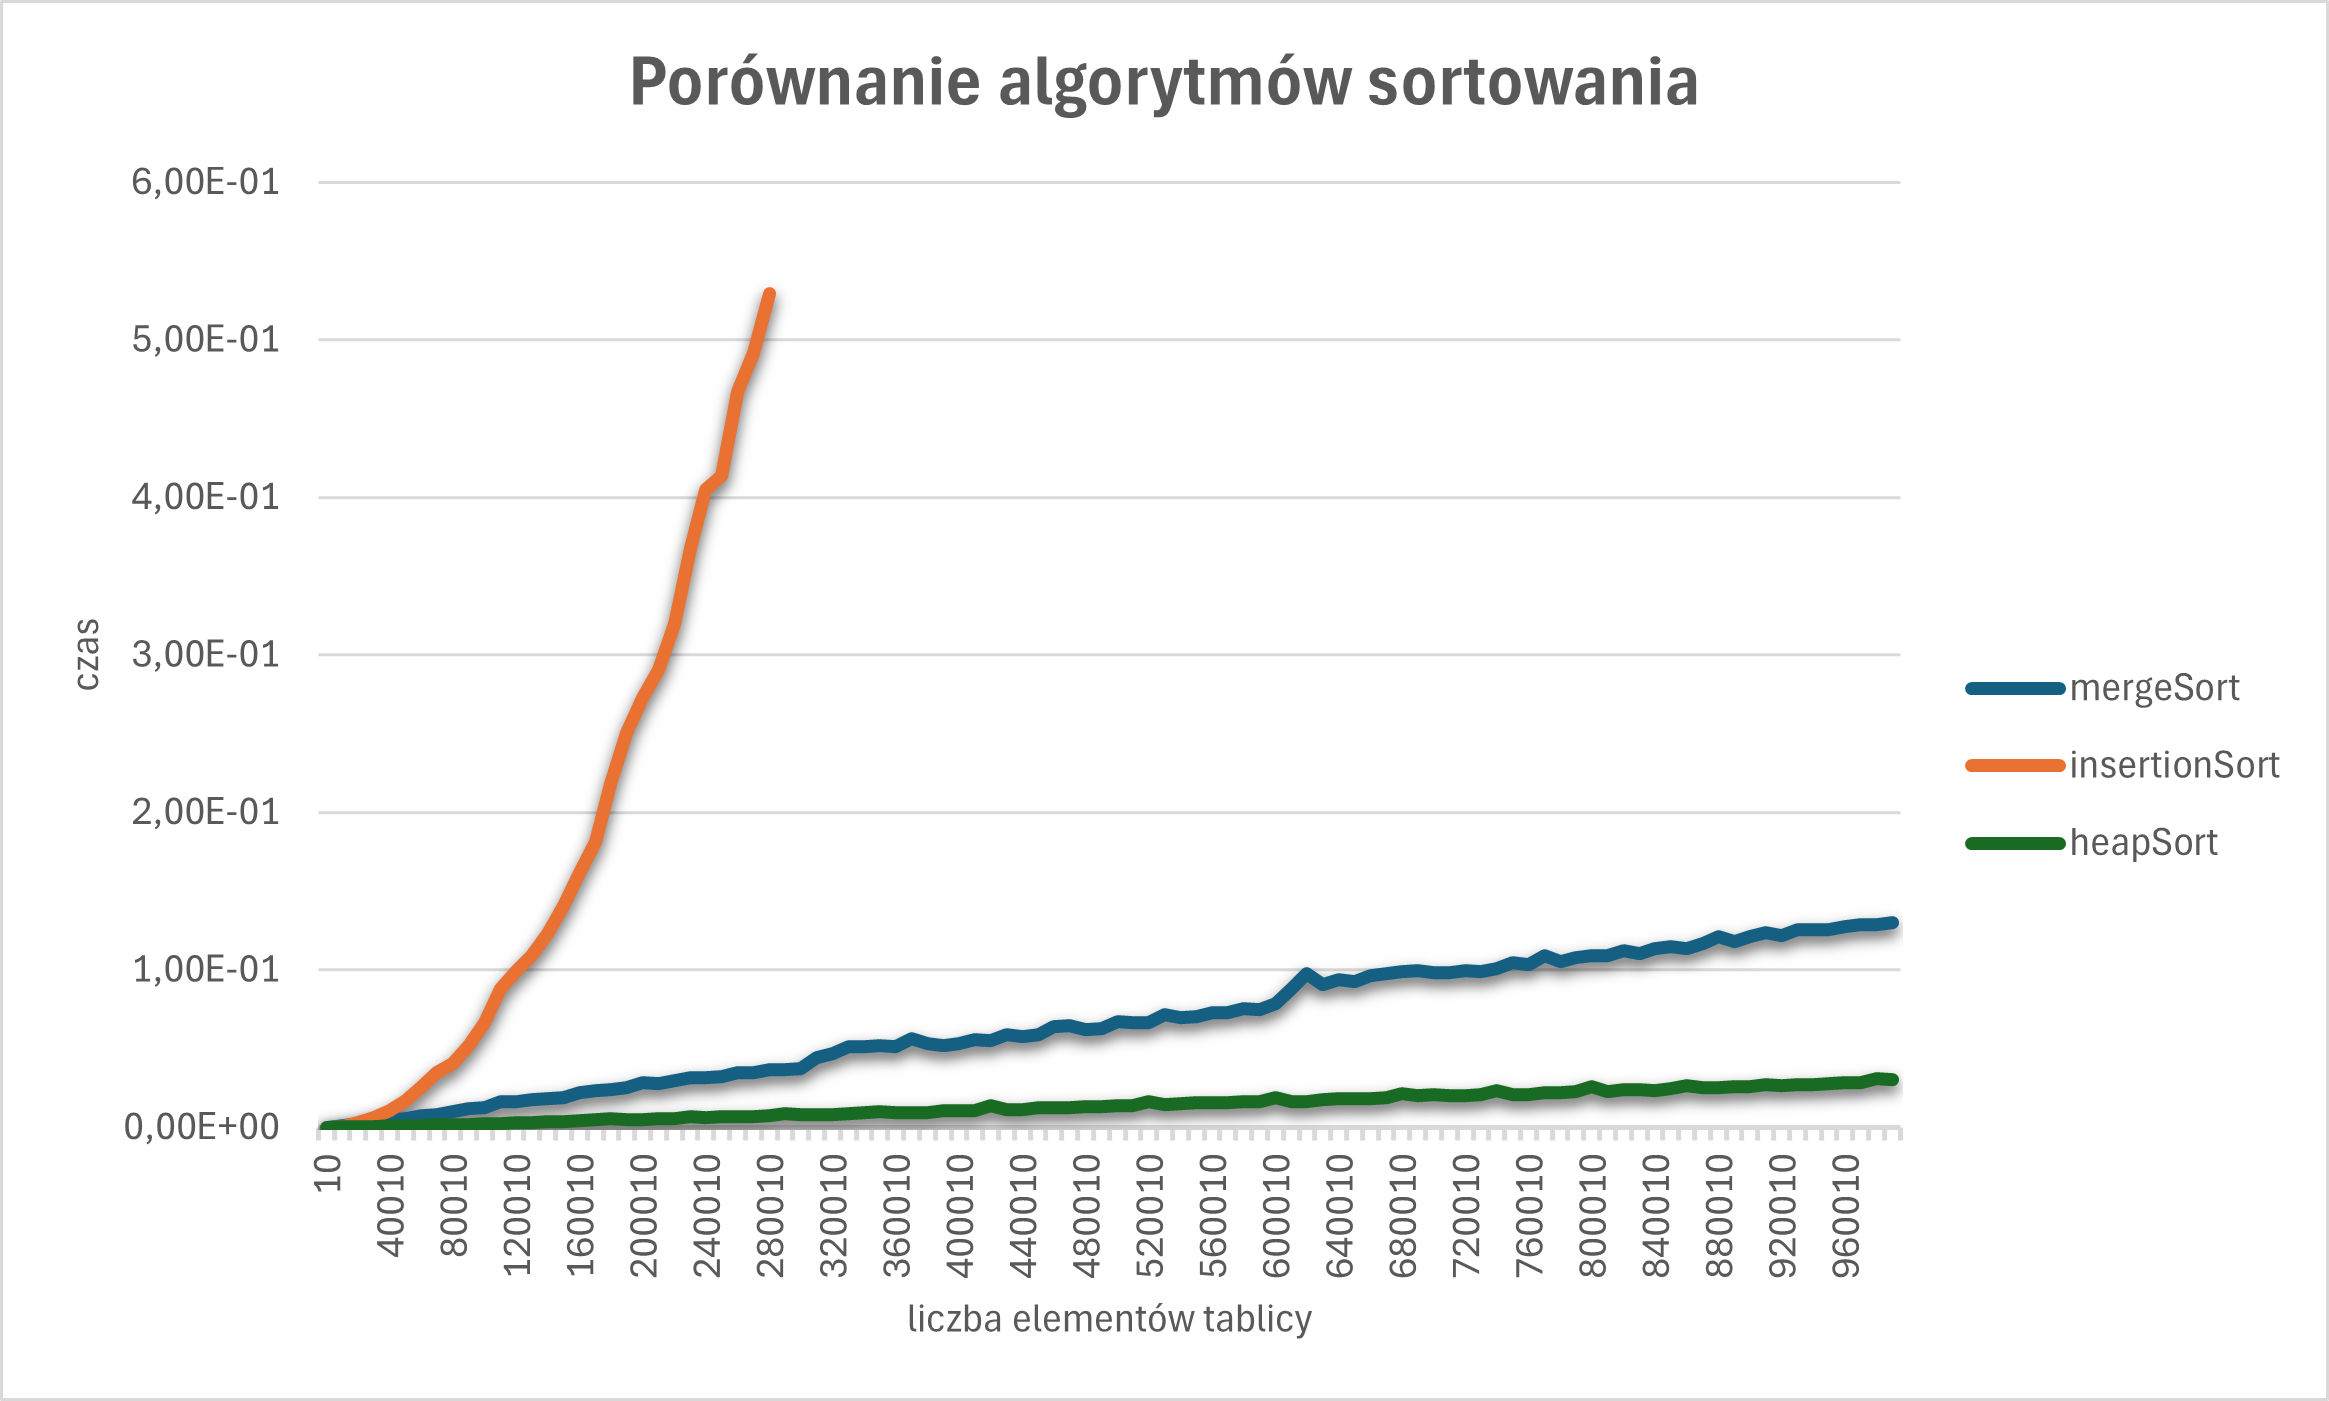
\includegraphics[width=\textwidth]{porowanie.png}
	\end{figure}
	
	Z wykresu możemy odczytać, że czas wykonania algorytmu \textit{insertion sort} jest znacząco większy od \textit{heap sort} oraz \textit{merge sort}. Jest to spowodowane faktem, że jego złożoność obliczeniowa wynosi $O(n^2)$, a nie $O(n \log n)$, jak w przypadku pozostałych algorytmów. Algorytm \textit{merge sort} jest porównywalnie czasochłonny co \textit{heap sort}; różnica widoczna na wykresie może wynikać z faktu, że w sortowaniu przez scalanie tworzymy pomocnicze tablice, zamiast operować na jednej, jak w przypadku sortowania przez kopcowanie.
	 
	 
	 
	
	\paragraph{Analiza liczby przypisań i porównań\\}
	W tabeli poniżej przedstawiono średnią ilość porównań i przypisań podczas wykonywania każdego sortowania, dla danego rozmiaru tablicy
	
	\begin{table}[H]
		\raggedright
		\begin{tabular}{|c|c|c|c|}
			\hline
			\textbf{Rozmiar} & \textbf{Insertion Sort} & \textbf{Merge Sort} & \textbf{Heap Sort} \\ \hline
			100 & \makecell{porównania: 5060 \\ przypisania: 5258} & \makecell{porównania: 771 \\ przypisania: 3105} & \makecell{porównania: 3175 \\ przypisania: 4509} \\ \hline
			1000 & \makecell{porównania: 526996 \\ przypisania: 528994} & \makecell{porównania: 10975 \\ przypisania: 40917} & \makecell{porównania: 48090 \\ przypisania: 69749} \\ \hline
			10000 & \makecell{porównania: 50457072 \\ przypisania: 50477070} & \makecell{porównania: 143615 \\ przypisania: 510837} & \makecell{porównania: 645690 \\ przypisania: 944142} \\ \hline
		\end{tabular}
		\caption{przypisania i porównania użyte w każdym sortowaniu}
	\end{table}
	
	Algorytm \textit{Insertion Sort} wykazuje najwyższą liczbę porównań i przypisań, szczególnie dla większych tablic, co wynika z jego złożoności $O(n^2)$. Z kolei \textit{Merge Sort} i \textit{Heap Sort}, obie o złożoności $O(n \log n)$, wykonują znacznie mniej operacji, co czyni je bardziej wydajnymi przy większych rozmiarach danych. \textit{Merge Sort} ma nieco niższą liczbę operacji niż \textit{Heap Sort}, co może się kłócić z danymi z pierwszego wykresu, natomiast może być to spowodowane faktem, że większym obciążeniem dla komputera jest przechowywanie tablic w pamięci niż wykonywanie operacji. 
	
	\newpage
	\section{Modyfikacje algorytmów}
	\paragraph{Sortowanie przez wstawianie (podwójne)\\}
	Pierwszym zmodyfikowanym algorytmem jest insertion sort. Zmiana polega na tym, że zamiast jednego elementu bierzemy dwa, porównujemy je ze sobą, a następnie za pomocą pętli while szukamy miejsca na wstawienie dla mniejszego elementu i powtarzamy to samo dla większego elementu. Musimy dodac także obsługę parzystych tablic gdzie ostatni element sortujemy tak jak w standardowej wersji.
	
	\begin{lstlisting}
for (int i = 1; i < n - 1; i += 2) {
	float key1, key2;
	if (A[i] < A[i + 1]) {
		key1 = A[i];
		key2 = A[i + 1];
	} else {
		key1 = A[i + 1];
		key2 = A[i];
	}
	
	// sortowanie mniejszego klucza
	int j = i - 1;
	while (j >= 0 && A[j] > key1) {
		A[j + 1] = A[j];
		j--;
	}
	A[j + 1] = key1;

	//sortowanie wiekszego klucza
	int j2 = i;
	while (j2 > j && A[j2] > key2) {
		A[j2 + 1] = A[j2];
		j2--;
	}
	A[j2 + 1] = key2;
}
	\end{lstlisting}
	
	Niestety nasza modyfikacja nie dała nam lepszych rezultatów, co możemy zobaczyć na poniższym wykresie:
	
	\begin{figure}[H]
		\centering
		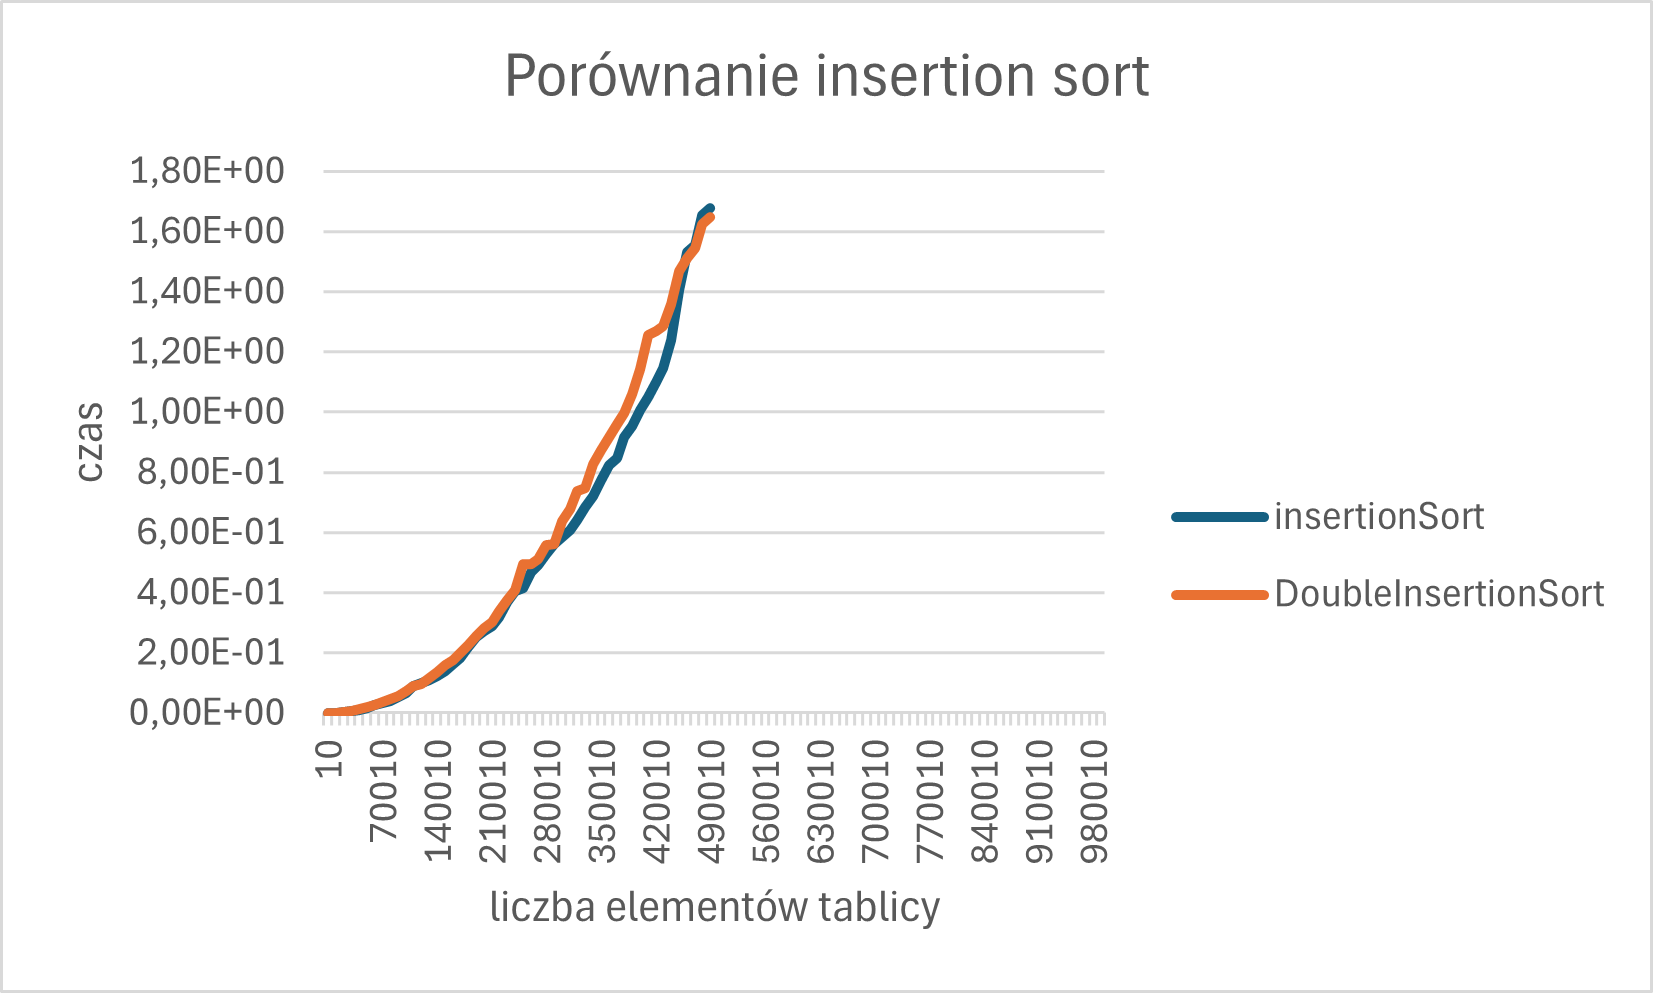
\includegraphics[width=\textwidth]{insertion.png}
	\end{figure}
	
	
	\paragraph{Potrójne sortowanie przez scalanie\\}
	W tej modyfikacji zamiast dzielić naszą tablice na dwie części, dzielimy na trzy, następnie porównujemy ze sobą elementy z trzech tablic i scalamy tak aby tworzyły coraz większe posortowane tablice. 
	
	\begin{lstlisting}
for (i = 0; i < n1; i++) {
	L[i] = A[i + p];
}
for (j = 0; j < n2; j++) {
	S[j] = A[j + s1 + 1];
}
for (h = 0; h < n3; h++) {
	R[h] = A[h + s2 + 1];
}

i = 0;
j = 0;
h = 0;

for (int l = p; l <= k; l++) {
	if (L[i] <= S[j] && L[i] <= R[h]) {
		A[l] = L[i];
		i++;
	} else if (S[j] <= L[i] && S[j] <= R[h]) {
		A[l] = S[j];
		j++;
	} else {
		A[l] = R[h];
		h++;
	}
}
	\end{lstlisting}
	\newpage
	Tutaj również nasza modyfikacja nie dała lepszych rezultatów, czas działania jest mniej więcej taki sam:
	
	\begin{figure}[H]
		\centering
		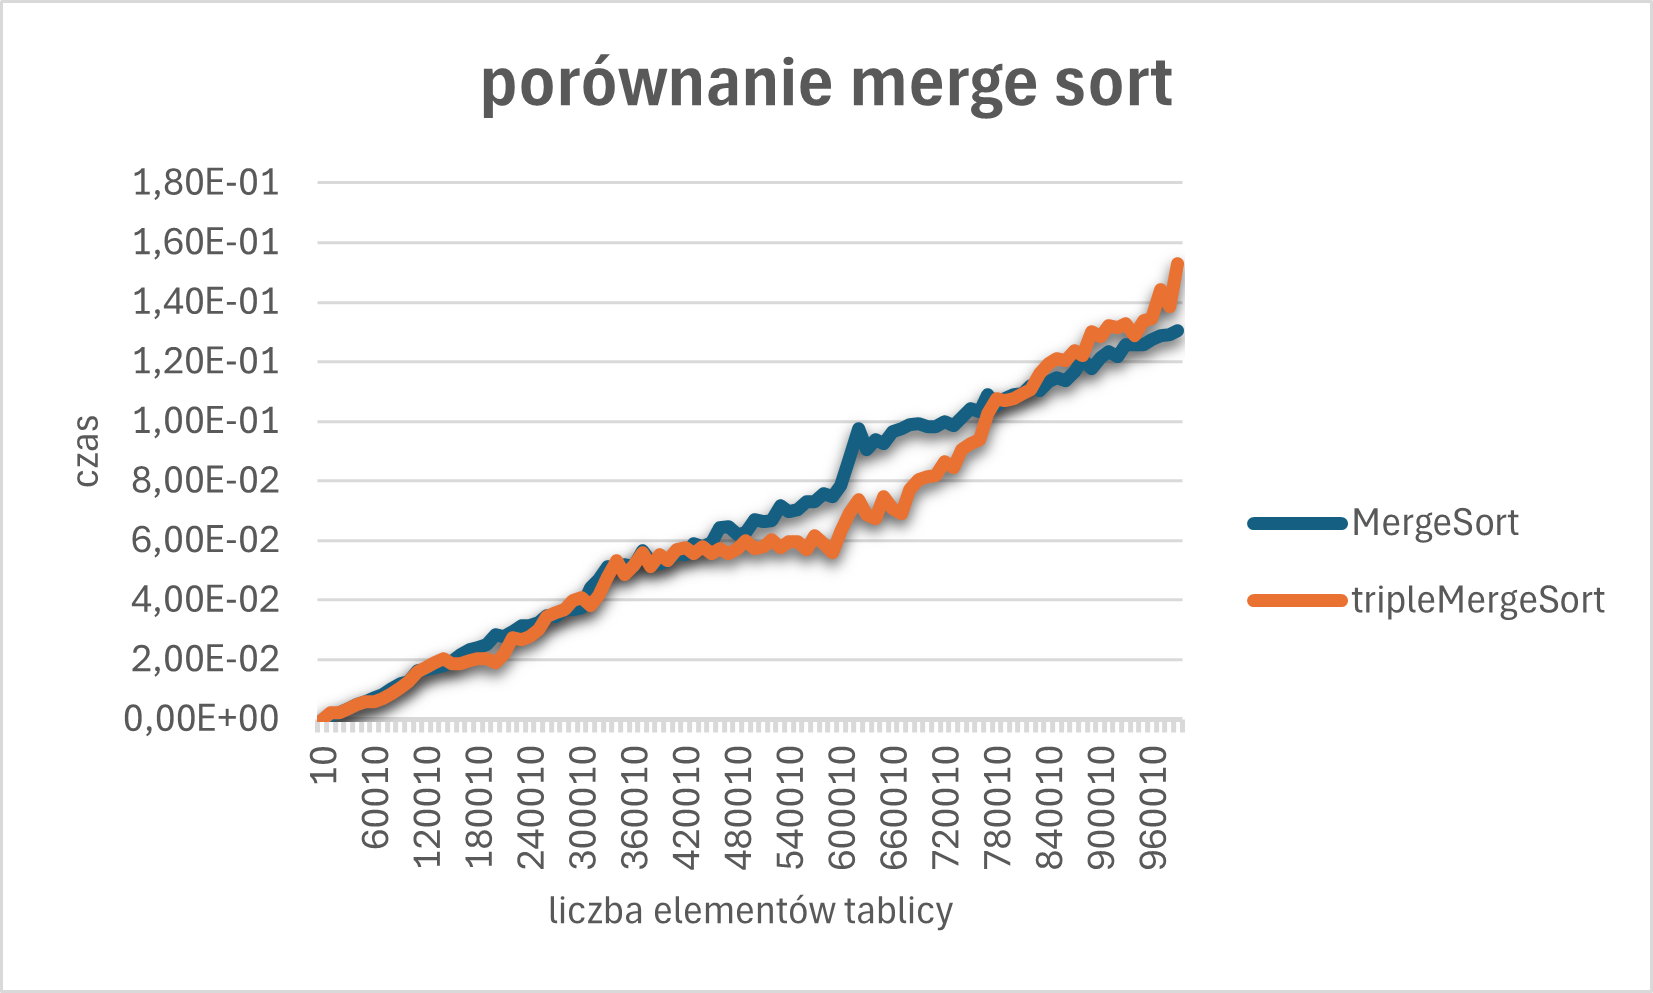
\includegraphics[width=\textwidth]{merge.png}
	\end{figure}
	
	\paragraph{Sortowanie przez kopcowanie ternarnie\\}
	Tutaj chcemy przede wszystkim użyć drzewka terarnego zamiast binarnego. Tworzymy takie drzewko, a następnie porównujemy korzeń z trzema dziećmi, tak aby na miejscu korzenia znalazł się największy element. Po każdym przejściu, tak jak w standardowej wersji, największy element przesuwamy na koniec gdzie tworzy się posortowana tablica.
	
	\begin{lstlisting}
void heapifyT(float A[], int n, int i) {
	int largest;
	int l = leftT(i);
	int m = middleT(i);
	int r = rightT(i);
	
	if (l < n && A[l] > A[i]) {
		largest = l;
	} else {
		largest = i;
	}
	
	if (m < n && A[m] > A[largest]) {
		largest = m;
	}
	
	if (r < n && A[r] > A[largest]) {
		largest = r;
	}
	
	if (i != largest) {
		float temp = A[i];
		A[i] = A[largest];
		A[largest] = temp;
		heapifyT(A, n, largest);
	}
}
	\end{lstlisting}
	
	W tym przypadku zwyczajny heap sort radzi sobie delikatnie gorzej co widać na dużych tablicach, jednak nie jest to znacząca różnica. 
	
	\begin{figure}[H]
		\centering
		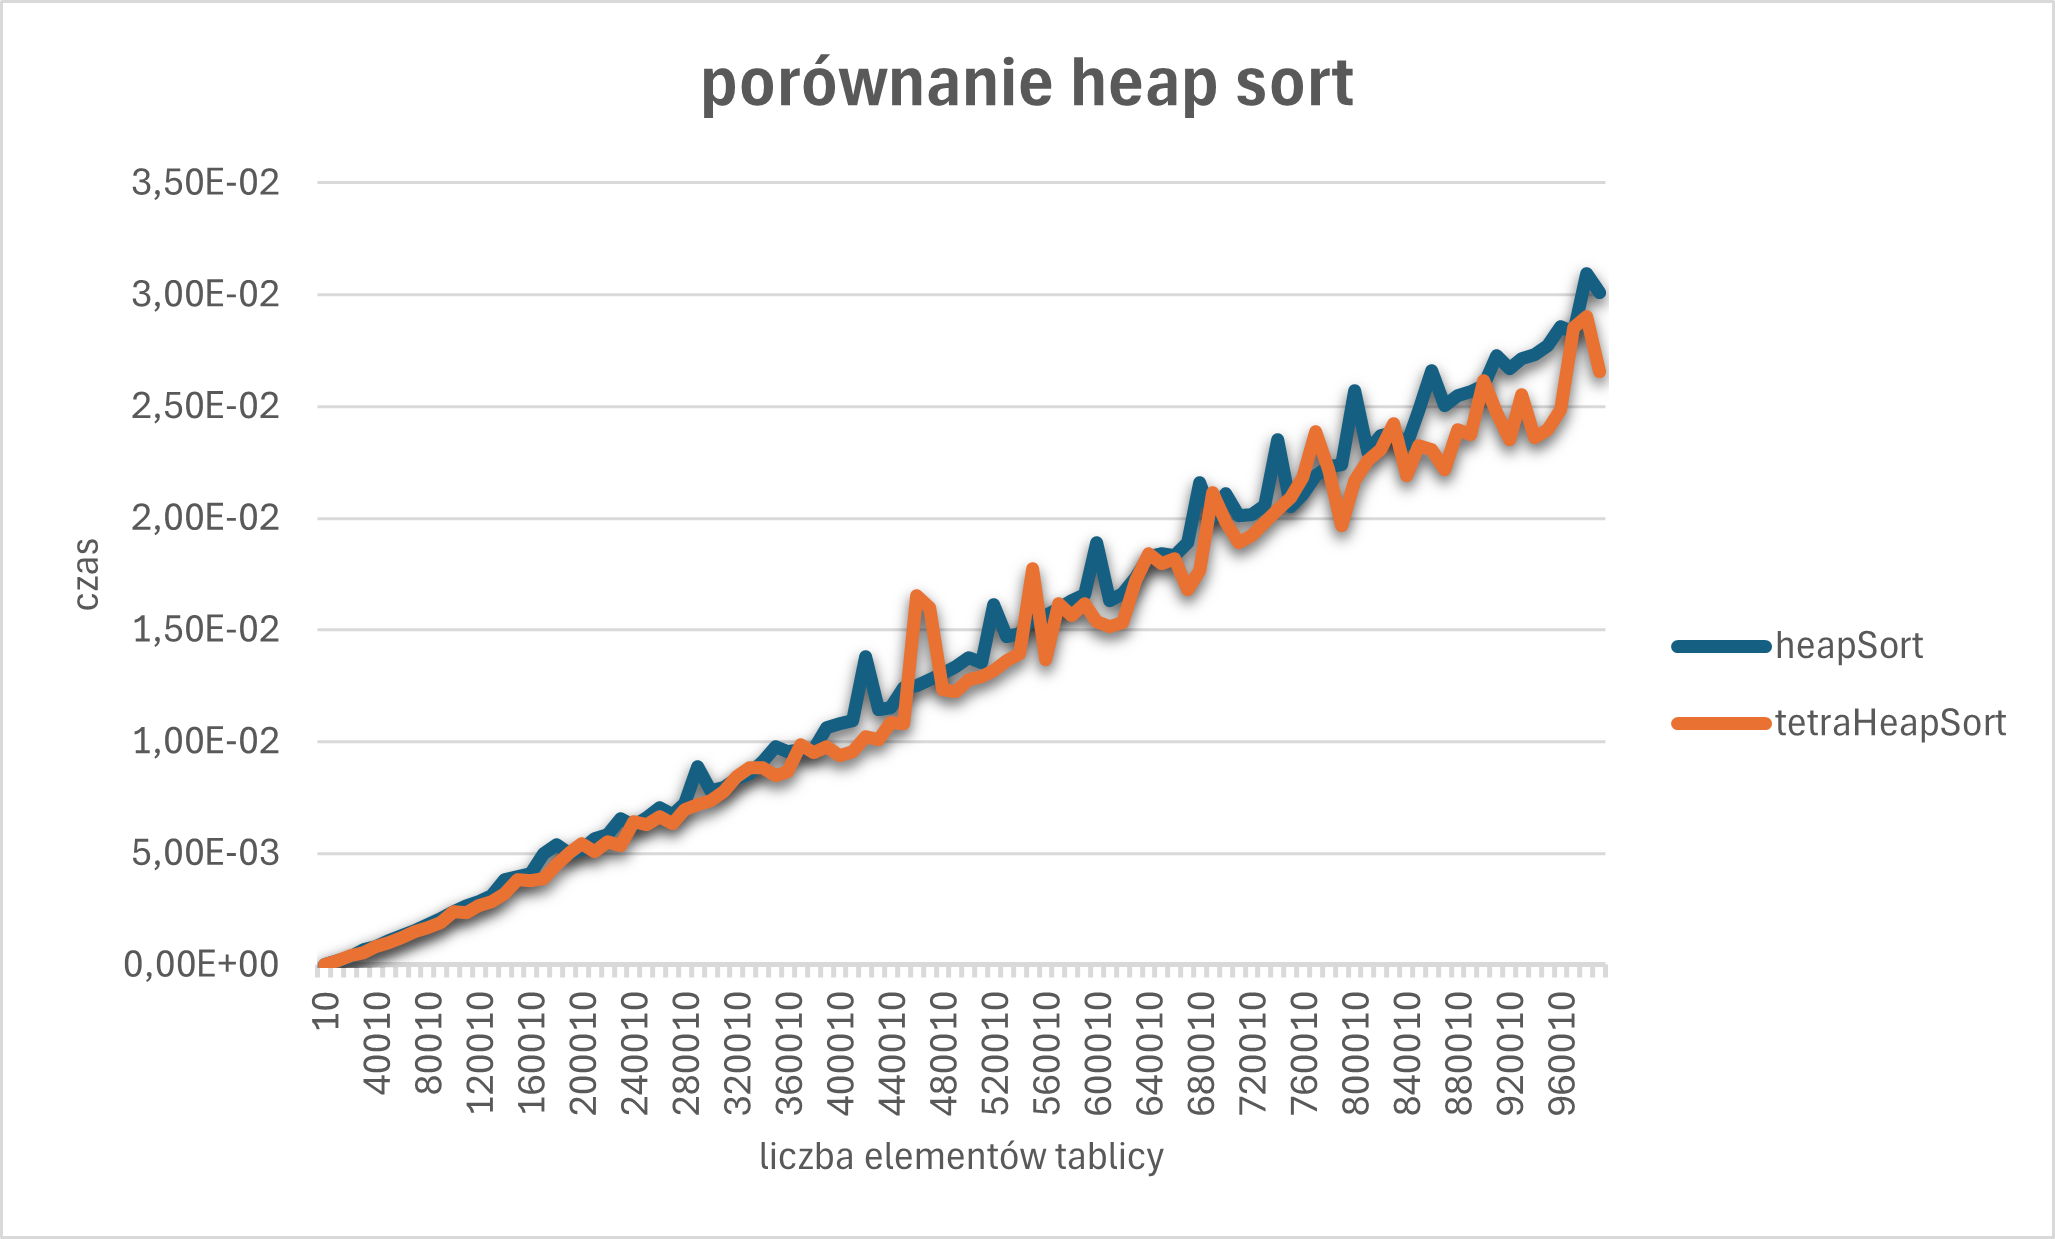
\includegraphics[width=\textwidth]{heap.png}
	\end{figure}
	
	
	\section{Wnioski}
	
	Po przeprowadzeniu testów na trzech algorytmach sortujących (\textit{Insertion Sort}, \textit{Merge Sort} i \textit{Heap Sort}), jak i na modyfikacjach, możemy wyciągnąć kilka  wniosków.
	
	\begin{itemize}
		\item \textbf{Wydajność algorytmów:} \textit{Insertion Sort} wypadł najgorzej, zwłaszcza przy większych zbiorach danych. Wynika to z tego, że ma on złożoność $O(n^2)$, przez co czas wykonania rośnie bardzo szybko w miarę wzrostu rozmiaru tablicy. Z kolei \textit{Merge Sort} i \textit{Heap Sort} mają złożoność $O(n \log n)$ i sprawdzają się dużo lepiej, szczególnie dla większych danych, \textit{Merge Sort} wypada trochę gorzej niż \textit{Heap Sort}, mimo ze ma mniej operacji, jednak może to być zależne od parametrów komputera na którym to testujemy.
		
		\item \textbf{Porównania i przypisania:} Jak widać, \textit{Insertion Sort} ma zdecydowanie najwięcej porównań i przypisań, zwłaszcza przy dużych tablicach. Na szczęście \textit{Merge Sort} i \textit{Heap Sort} wykonują ich mniej, co sprawia, że są po prostu bardziej wydajne przy dużych zbiorach danych.
		
		\item \textbf{Zmodyfikowane algorytmy:} Zmodyfikowane wersje algorytmów, takie jak podwójne sortowanie przez wstawianie, potrójne sortowanie przez scalanie i ternarne sortowanie przez kopcowanie, niestety nie dały lepszych rezultatów. Wydaje się, że nie zmieniając zasadniczo złożoności algorytmów, nie osiągnęliśmy poprawy, a czas wykonania pozostał mniej więcej taki sam jak w przypadku wersji standardowych. Zatem można powiedzieć, że najlepiej pozostać przy klasycznych wersjach algorytmów\\
		
	\end{itemize}
	
	\textbf{Podsumowując } Jeśli chodzi o wybór algorytmu do dużych zbiorów danych, \textit{Merge Sort} i \textit{Heap Sort} to zdecydowanie lepszy wybór niż \textit{Insertion Sort}. Zmodyfikowane wersje algorytmów (np. z większą liczbą elementów do porównań) nie sprawdziły się i nie poprawiły znacząco wyników. Można powiedzieć, że proste algorytmy takie jak \textit{Merge Sort} są po prostu wystarczająco dobre do większości zastosowań.
	
\end{document}
